% Requires \usepackage{tikz}. Three diagnostic input signals (i)--(iii); each row
% of \cref{tab:divergence-profile} names its signal label next to the test
% formula. Visual key (see caption): samples spaced EVENLY by index; the t-axis
% gives each sample's real time; dashed line = value 0; x=blue, y=red; orange
% ring = the readout time whose robustness Table 2 reports.
%
% TO EDIT a panel: set its value range [\vmin,\vmax] (mapped to the band
% [0,\sigH]) and list the samples as index/value and the ticks as index/realtime.
% The y-coordinate is computed from the actual value, so only the numbers below
% change. \vmin/\vmax also fix where the dashed zero line lands.
\def\sigdx{0.85}      % horizontal spacing between consecutive samples (by index)
\def\sigH{1.10}       % value-band height: \vmin maps to 0, \vmax maps to \sigH
\def\sigaxisy{-0.16}  % time-axis y
\def\sigticky{-0.24}  % tick-bottom y
\definecolor{readoutorange}{RGB}{225,100,0}
\newcommand{\sigX}[1]{#1*\sigdx}                            % x for a sample index
\newcommand{\sigY}[1]{(#1-(\vmin))/((\vmax)-(\vmin))*\sigH} % y for a value

\begin{tabular}{@{}c@{\hspace{4.5em}}c@{\hspace{4.5em}}c@{}}
% ---- (i) signal model: x = 1, 1, -9 at t = 0, 1, 9; readout at t = 0 ----
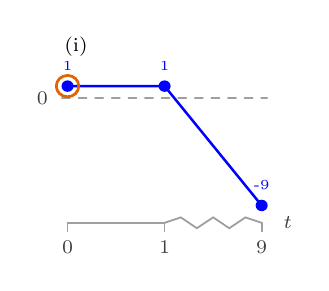
\begin{tikzpicture}[xscale=1.45,yscale=1.3775,baseline={(0,0.30cm)},line width=0.9pt,line cap=round]
  \def\vmin{-9}\def\vmax{1}
  \def\xpts{0/1, 1/1, 2/-9}
  \draw[gray!75,dashed,line width=0.45pt] (-0.05,{\sigY{0}}) -- ({\sigX{2}+0.05},{\sigY{0}});
  \node[font=\scriptsize,black!75,anchor=east] at (-0.08,{\sigY{0}}) {0};
  \draw[gray!75,line width=0.55pt] ({\sigX{0}},\sigaxisy) -- ({\sigX{1}},\sigaxisy);
  \draw[gray!75,line width=0.65pt] ({\sigX{1}},\sigaxisy) -- (0.992,-0.110) -- (1.133,-0.210) -- (1.275,-0.110) -- (1.417,-0.210) -- (1.558,-0.110) -- ({\sigX{2}},\sigaxisy); % time gap 1->9
  \foreach \i/\rt in {0/0, 1/1, 2/9} {
    \draw[gray!75,line width=0.65pt] ({\sigX{\i}},\sigaxisy) -- ({\sigX{\i}},\sigticky);
    \node[font=\scriptsize,black!75,anchor=north] at ({\sigX{\i}},{\sigticky+0.01}) {\rt};
  }
  \node[font=\scriptsize,black!75,anchor=west] at ({\sigX{2}+0.10},\sigaxisy) {$t$};
  \foreach \i/\v [count=\n] in \xpts { \coordinate (p\n) at ({\sigX{\i}},{\sigY{\v}}); }
  \draw[blue] (p1)--(p2)--(p3);
  \foreach \i/\v [count=\n] in \xpts {
    \fill[blue] (p\n) circle (1.5pt);
    \node[font=\tiny,blue,anchor=south] at ({\sigX{\i}},{\sigY{\v}+0.05}) {\v};
  }
  \draw[readoutorange,line width=1.0pt] (p1) circle (2.8pt);
  \node[font=\scriptsize,anchor=base west] at (-0.12,1.42) {(i)};
\end{tikzpicture}
&
% ---- (ii) signal beyond horizon: x = 5, 3 at t = 0, 1; readout at t = 0 ----
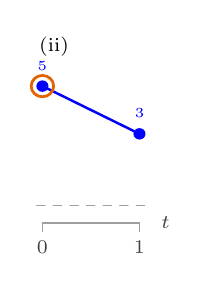
\begin{tikzpicture}[xscale=1.45,yscale=1.3775,baseline={(0,0.30cm)},line width=0.9pt,line cap=round]
  \def\vmin{0}\def\vmax{5}
  \def\xpts{0/5, 1/3}
  \draw[gray!75,dashed,line width=0.45pt] (-0.05,{\sigY{0}}) -- ({\sigX{1}+0.05},{\sigY{0}});
  \draw[gray!75,line width=0.55pt] ({\sigX{0}},\sigaxisy) -- ({\sigX{1}},\sigaxisy);
  \foreach \i/\rt in {0/0, 1/1} {
    \draw[gray!75,line width=0.65pt] ({\sigX{\i}},\sigaxisy) -- ({\sigX{\i}},\sigticky);
    \node[font=\scriptsize,black!75,anchor=north] at ({\sigX{\i}},{\sigticky+0.01}) {\rt};
  }
  \node[font=\scriptsize,black!75,anchor=west] at ({\sigX{1}+0.10},\sigaxisy) {$t$};
  \foreach \i/\v [count=\n] in \xpts { \coordinate (p\n) at ({\sigX{\i}},{\sigY{\v}}); }
  \draw[blue] (p1)--(p2);
  \foreach \i/\v [count=\n] in \xpts {
    \fill[blue] (p\n) circle (1.5pt);
    \node[font=\tiny,blue,anchor=south] at ({\sigX{\i}},{\sigY{\v}+0.05}) {\v};
  }
  \draw[readoutorange,line width=1.0pt] (p1) circle (2.8pt);
  \node[font=\scriptsize,anchor=base west] at (-0.12,1.42) {(ii)};
\end{tikzpicture}
&
% ---- (iii) robustness at horizon: x = y = 5, 5, -3 at t = 0, 1, 2; readout at t = 2 ----
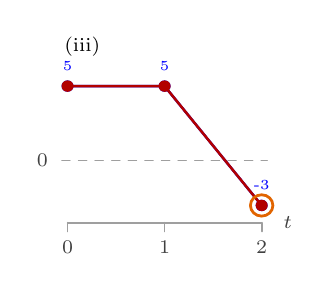
\begin{tikzpicture}[xscale=1.45,yscale=1.3775,baseline={(0,0.30cm)},line width=0.9pt,line cap=round]
  \def\vmin{-3}\def\vmax{5}
  \def\xpts{0/5, 1/5, 2/-3}
  \draw[gray!75,dashed,line width=0.45pt] (-0.05,{\sigY{0}}) -- ({\sigX{2}+0.05},{\sigY{0}});
  \node[font=\scriptsize,black!75,anchor=east] at (-0.08,{\sigY{0}}) {0};
  \draw[gray!75,line width=0.55pt] ({\sigX{0}},\sigaxisy) -- ({\sigX{2}},\sigaxisy);
  \foreach \i/\rt in {0/0, 1/1, 2/2} {
    \draw[gray!75,line width=0.65pt] ({\sigX{\i}},\sigaxisy) -- ({\sigX{\i}},\sigticky);
    \node[font=\scriptsize,black!75,anchor=north] at ({\sigX{\i}},{\sigticky+0.01}) {\rt};
  }
  \node[font=\scriptsize,black!75,anchor=west] at ({\sigX{2}+0.10},\sigaxisy) {$t$};
  \foreach \i/\v [count=\n] in \xpts { \coordinate (p\n) at ({\sigX{\i}},{\sigY{\v}}); }
  \draw[blue] (p1)--(p2)--(p3);
  \foreach \i/\v [count=\n] in \xpts {
    \fill[blue] (p\n) circle (1.5pt);
    \node[font=\tiny,blue,anchor=south] at ({\sigX{\i}},{\sigY{\v}+0.05}) {\v};
  }
  \draw[red!70!black] (p1)--(p2)--(p3);
  \foreach \i/\v [count=\n] in \xpts { \fill[red!70!black] (p\n) circle (1.5pt); }
  \draw[readoutorange,line width=1.0pt] (p3) circle (2.8pt);
  \node[font=\scriptsize,anchor=base west] at (-0.12,1.42) {(iii)};
\end{tikzpicture}
\\
\end{tabular}
